% UNIT: Psychology of Concepts and Categories
\chapter{Psychology of concepts and categories}
\label{chap:concepts_categories}

In this Chapter we discuss about categories in sensation/perception (non-semantic categories, Section \ref{sec:categories}) and conceptual structure (words and concepts, Section \ref{sec:conceptual_structure}).

\section{Categories and categorical perception}
\label{sec:categories}

Categorical perception is the phenomenon in which people perceive stimuli from different categories as more different from each other than stimuli from within the same category. This is useful as it introduces invariance in response with respect to a functionally defined category, allowing for rapid prediction, efficient memory, and compression.

\boxc{How we know categorical representation exists}{
A demonstrating experiment consists in:
\begin{itemize}
    \item selecting a set of stimuli that uniformly covers a certain physical domain (e.g., sound freq 100Hz-8000Hz),
    \item select an objective distance measure so that the space is partitioned in intervals; e.g., distance in frequency space (applicable to both sounds and colors),
    \item select a method for operationalizing human similarity (e.g., similarity judgments, generalization, confusion [same/different]),
    \item in one procedure, assign all stimuli to categories (e.g., assign all stimuli to color names); in a second, obtain similarity judgments for within-category vs.~between-category pairs, or ask for categorization, and evaluate if the boundary is fuzzy or not (e.g., how much objects are considered similar when belonging to the same category, and when to different categories).
\end{itemize}
}

\subsection{Categorical perception in audition}
In auditory stimuli, there is discrimination between speech sounds. People have a sharper discrimination boundary between sounds that are perceived as belonging to different phonetic categories than between sounds that are perceived as belonging to the same category.
For experimenting, we use as objective dimension the \textbf{Voice Onset Time} (VOT) of consonants (i.e., the timespan between the start of the consonant and the start of sound emitted by vocal cords). The discrimination performance is simply a ``same/different" judgment. We present consonants such as /b/ and /p/. A fixed-size physical difference in VOT, that is easily discriminated when it straddles the boundary between two categories (labeled as /b/ or /p/), produces \textit{chance} discrimination performance when both tokens come from the same category (either both /b/ or both /p/); results are in Fig.~\ref{fig:bapa}.

\textbf{Within phonetic category}, two \textbf{different stimuli sound the same} (see \notedv Eimas et al. (1971)).\\

Prior categories aid online processing via categorical perception, in a sort of \textit{experience-dependent learning}; related phenomena are:
\begin{itemize}
    \item \textit{Change deafness}, Vitevitch (2003): participants repeat words presented by a speaker. Halfway through study, the speaker changed. Only 40\% of participants noticed the change.
    \item \textit{Sine-wave speech}: phonetic categories/expectations can be considered \textit{priors} on sounds, impacting whether a stimulus is perceived as speech (e.g., if you previously listen to a voice and then hear a sound which is not speech, but has some correlation to the previous voice, you can ``hear" the words\footnote{\url{https://users.sussex.ac.uk/~cjd/SWS/}}).
    \item \textit{McGurk Effect}: the categorization of sounds is not only an auditory task, since our brain combines multimodal inputs (e.g., also from vision\footnote{\url{https://www.youtube.com/watch?v=PWGeUztTkRA&t=49s}}).
\end{itemize}

\begin{figure}
    \centering
    \captionsetup{width=.8\linewidth}
    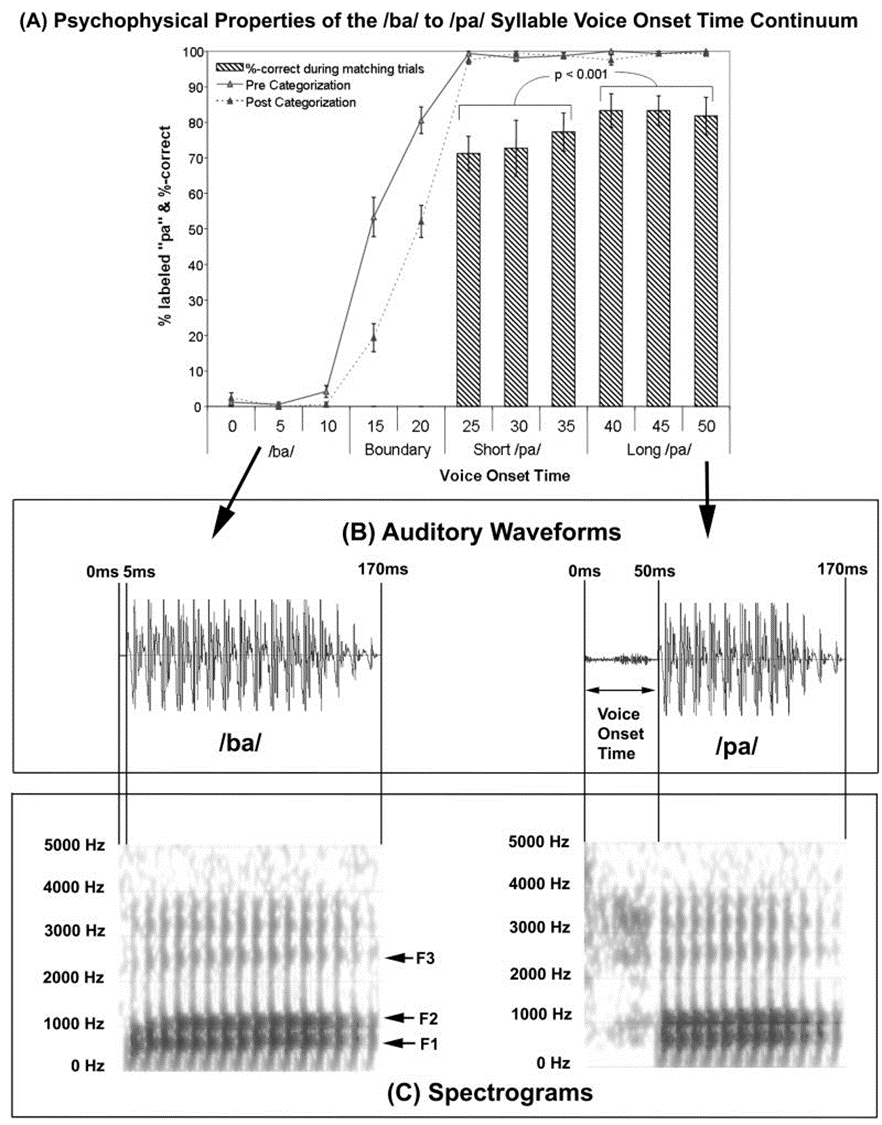
\includegraphics[width=0.8\linewidth]{images/vot.png}
    \caption{For the experiment, they created a range of stimuli with VOT between 5ms and 50ms (which are the standard values for respectively /ba/ and /pa/).
    In \textbf{(A)} are the results, with the percentage of responders hearing a /pa/ sound. We see the shift is between 10ms and 25ms}
    \label{fig:bapa}
\end{figure}

\boxl{Eimas et al. (1971)}{
They observed 4-month old sucking rate on pacifier (notice that a higher rate is interpreted as more surprise/interest). They examined the rate as function of relation between current and previously heard stimuli, in particular they presented two stimuli with VOT differing by 20ms. In one condition (labeled ``D") the difference straddled (on two sides of) the border of a phonetic boundary (stimuli perceived as ``b" and ``p" by adults). In another condition ``S" they belonged to the same phonetic category.\\

See Fig.~\ref{fig:eimas} for more details.
}

\begin{wrapfigure}[20]{r}{0pt}
  \begin{subfigure}{.22\textwidth}
  \centering
    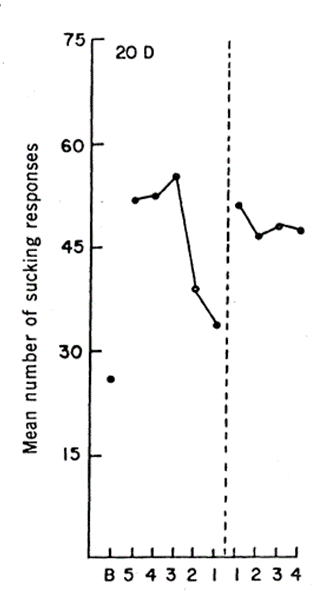
\includegraphics[height=5.5cm]{images/eimas_a.png}
    \caption{}
  \end{subfigure}%
  \begin{subfigure}{.2\textwidth}
  \centering
    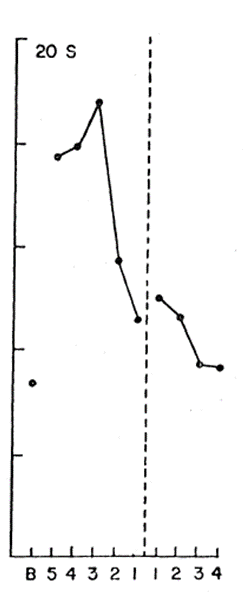
\includegraphics[height=5.5cm]{images/eimas_b.png}
    \caption{}
  \end{subfigure}
  \caption{5 min of habituation precede a 20ms VOT change, either within the same \textbf{(a)} or across \textbf{(b)} phonetic category; habituation consists in hearing the /ba/ sound. This proves how 4-month-old children already have the auditory \textbf{categorization} enabling them to distinguish between /b/ and /p/ sounds.}
    \label{fig:eimas}
\end{wrapfigure}

Brain areas coding for \textbf{low-level} representations are \textbf{not influenced} by such categorization, while those coding for high-level representations are.

\subsection{Categorical perception in vision}
In categorical perception for color, discrimination of items that cross category boundaries is better (faster, more accurate) than when the items are within the same color category. Notice that color category is \textbf{linguistic} \notet.
For example, it is easier to distinguish between a green stimulus and a blue stimulus than between two stimuli within the same category (two shades of green), who are \textbf{spaced at the same distance}.
\osst{Practical note: color differences in terms of discriminability can be equated across between-category and within-category comparisons by using the \textit{Commision Internationale de L'Eclairage} (CIE) values.}

\textbf{Color categories are not universal}, and thus \textbf{categorical perception depends on language} (see \notedv Robertson et al. (2000)).

\boxl{Robertson et al. (2000)}{
The stone-age tribe Berinmo uses ``\textit{nol}” as the color name that in English falls under both green and blue, so they have no categorical perception at the boundary between green and blue (no boundary in their language). On the contrary, they have a category boundary between ``\textit{nol}" and ``\textit{wor}'' that does not exist in English as both sides are green. Berinmo people exhibit better discrimination of 32 cross-category items than 32 within-category items at the boundary between \textit{nol} and \textit{wor}. English speakers do not show categorical perception at this boundary.
}

\section{Conceptual structure}
\label{sec:conceptual_structure}

\subsection{Theory on words and concepts}
The typical approach is to assume that words are associated with concepts or a network of conceptual representations.
We need to first have a good theory of what the conceptual structure is like, and then we can see how this structure is used to represent meaning when referred to by words.
Ultimately, a word is a sound or written pattern, and it is generally assumed that a single word corresponds to a single concept (this assumption would help with word-embedding models), but there are complications.

There is evidence proving that \textit{form-to-meaning mapping} is not \textit{1-to-1}. We encounter \textbf{polysemy}: a phenomenon where a single word can have multiple meanings depending on the context in which it is used, such as ``cinema" which can refer to different things in different contexts (e.g., \textit{American cinema is naïve} vs \textit{This cinema is ugly}).

According to Murphy, it is impossible for a single concept to fully capture the meaning of a polysemous word; the process of \textbf{meaning extension} is not a result of \textit{natural change} (chaining) but a matter of \textbf{online derivation}. Online derivation does not prevent information from also being stored somewhere, at least for a short time, in order to understand the nearby context more effectively. Indeed, Klein and Murphy (2001) found evidence suggesting that the different senses of polysemous words can be stored, as they observed priming effects when a word was used twice in the same sense, and interference effects when the sense was switched.

Another possibility is that a word specifies a set of potentials that is then refined by context to determine which sense is intended (i.e., a word opens a ``tree" of possible meanings which is pruned to select the right meaning according to the context).\\

To put it in a nutshell: \textbf{words are not concepts}. Such distinction between \textit{meaning} and \textit{lexical form} is also proven by \textit{anomia}, which is a type of \textit{aphasia} that results in the inability to retrieve the lexical form of a concept for production, even though the ability to recognize or define the term is maintained.

\subsection{Focusing on conceptual structure}
Understanding word meaning requires understanding the organization of conceptual structure in the mind-brain. Concepts represent our knowledge of things in the world and enable us to identify things, infer features, or know how to interact with them. Access to conceptual structure can be achieved through various means, including words, pictures, or music \notet. The study of conceptual structure or ``semantic memory" should be independent of what governs word meaning or how word meanings are accessed through language. Much of this psychology work focuses on how people represent categories, with classical experiments focused on artificial, non-linguistic categories to see how people ``summarize" those. We will not get into that, but be aware of the link.
In much of the literature, concepts are studied by using words, assuming that words map onto conceptual knowledge and are a reasonable ``proxy" for studying relations between concepts.

\osst{Access to conceptual structure is more rapid when people are presented an image, than when presented a word (for the same concept). There are studies showing that music also influences the time of access to conceptual structures.}

\subsubsection{The classic view of word meaning}
In the classic view \textit{word} and \textit{concept} are the same, and the word's meaning is a \textbf{definition}. Definitions are sets of necessary conditions that are jointly sufficient: every object is \textbf{either within a category or not} (e.g., \textit{Bachelor = Man, unmarried}).
This classical view of \textit{concept structure} (word meaning) implies that there are no different levels of category membership (all members are equivalent to others), so what people learn is the set of defining features. This has the advantage of supporting hierarchical structure and inheritance.


\subsection{Representing the meaning of concepts in the brain}

\begin{wrapfigure}[15]{r}{0pt}
  \centering
  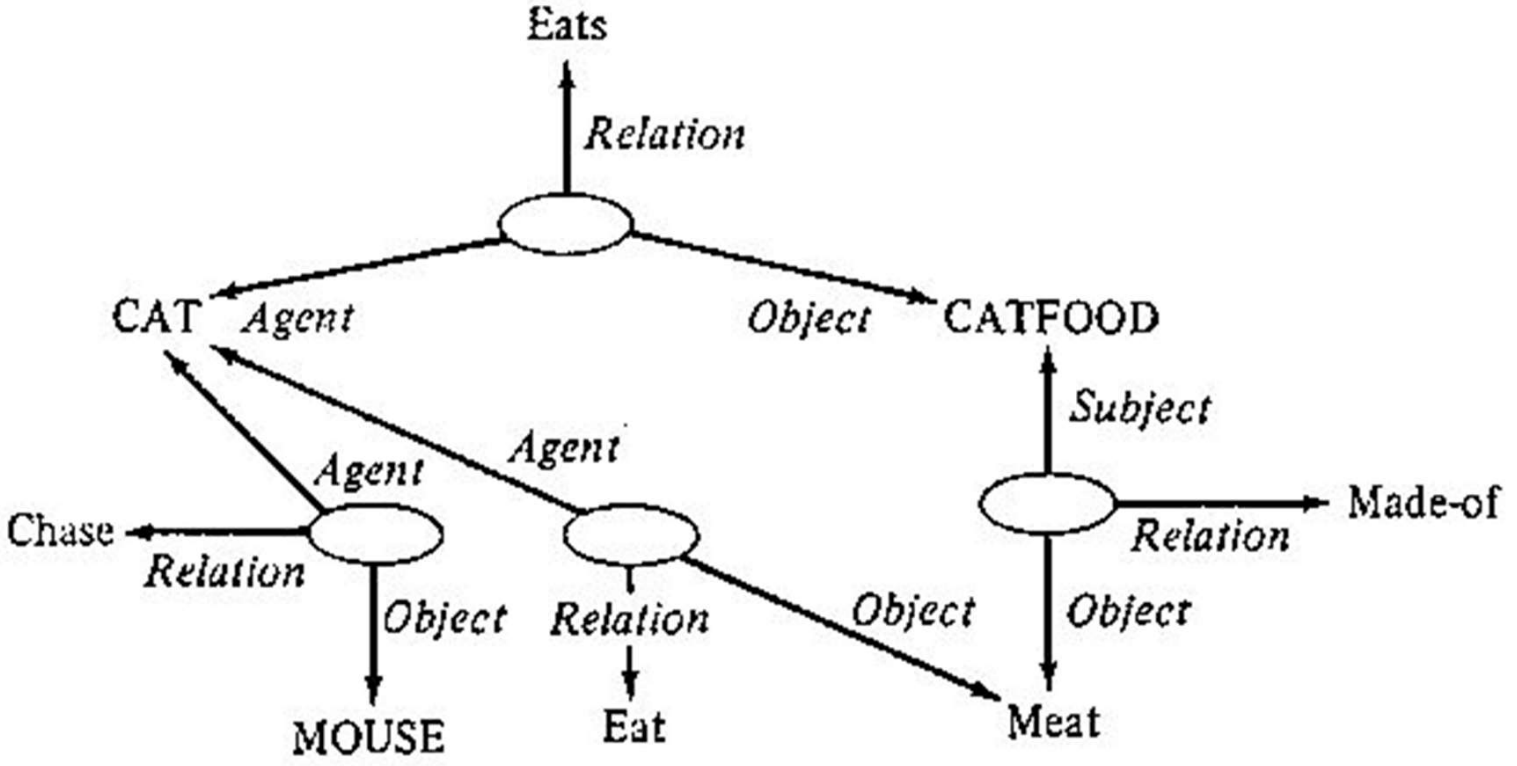
\includegraphics[width=0.6\textwidth]{images/cat_pn.png}
  \caption{A partial representation of ``cat" in memory.}
  \label{fig:cat_pn}
\end{wrapfigure}

We first introduce \textbf{propositional networks}.
A concept has a definition (e.g., \textit{Dog: a member of the canine species, that is domesticated}), it can inherit the default features of the parent class (\textit{canine}) and add a few exceptions if non-default. 
Then the parent classes in the taxonomy are defined (\textit{canine}, then \textit{mammal}, \textit{vertebrate}, \textit{animal}, \textit{organism}, etc).
At the end, some reference to visual features is added.

An example of representation in memory is provided in Fig.~\ref{fig:cat_pn}, while Fig.~\ref{fig:animal_pn} shows a propositional network.

\subsubsection{Propositional networks as psych model}

\begin{figure}
    \centering
    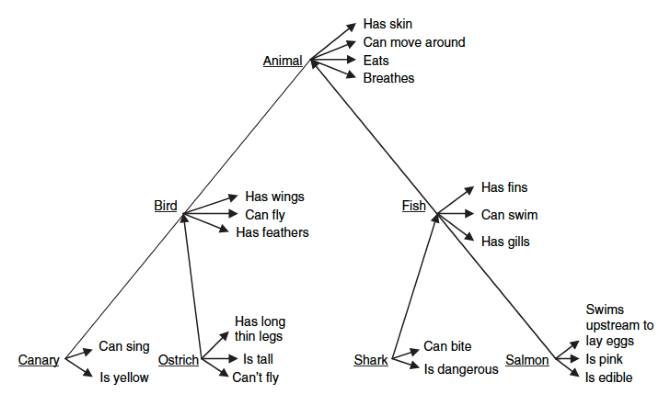
\includegraphics[width=0.7\linewidth]{images/animal_pn.png}
    \caption{Propositional network used by Collins and Quillian (1969).}
    \label{fig:animal_pn}
\end{figure}
Collins and Quillian (1969) study of conceptual structure involved \textbf{measuring response latencies for statements} such as ``Robins \textit{eat worms}/\textit{have feathers}/\textit{have skin}". The study proposed that \textbf{some features of a concept are directly stored} while \textbf{others are inferred through inheritance}. For example, the feature ``have skin" can be inferred after traversing three links in the ISA hierarchy: ``is bird", ``is animal", ``animals have skin". On the other hand, ``have feathers" can be inferred from a lower level in the hierarchy.
The latencies of affirmative responses were expected to reflect this distinction (see the results in Tab.~\ref{tab:collins}). One \textbf{question} that the study raises is whether these hierarchies are \textbf{pre-represented in memory} or whether they are \textbf{formed \textit{on the fly}} when people are asked questions.\\

\begin{table}[t]
    \centering
    \captionsetup{width=.8\linewidth}
    \begin{tabular}{lr}
        \hline
        Sentence & Latency \\
        \hline
        Robins \textit{eat worms} & 1310 ms \\
        Robins \textit{have feathers} & 1380 ms \\
        Robins \textit{have skin} & 1470 ms \\
        \hline
    \end{tabular}
    \caption{Verification time of affirmative responses. Even though the difference in timing seems to be small, it is actually massive (there are brain processes taking only 5 ms, so 70 ms is a lot). To measure the latency, EEG was used.}
    \label{tab:collins}
\end{table}

Propositional networks, however, present some problems:
\begin{itemize}
    \item \textbf{Verification time is not solely determined by hierarchical relations}, but is \textbf{also influenced by the frequency of encountered statements}. For instance, ``apples are eaten" is verified faster than ``apples have dark seeds."
    \item The propositional network approach suggests that verification times should increase as the number of ISA links traveled increases. However, people are \textbf{faster to verify} ``\textbf{dogs are animals}" \textbf{than} ``\textbf{dogs are mammals}".
    \item The approach expects \textbf{clear logical inferences}, such as ``if A is a B and B is a C, then A is a C." But this \textbf{assumption has been challenged}. For example, while a car seat is a seat and people agree that seats are furniture, car seats are not considered furniture.
\end{itemize}

\subsubsection{Prototypes}
Rosch (1973) proposed an alternative to propositional networks. He argued against the idea of ``sets of necessary and sufficient features”, taking the example of ``game" (there is no set of necessary and sufficient conditions that is in common to all games. Team? Yes/no. Physical skill? Yes/no etc).
Instead, what makes all games ``games" is their \textbf{family-resemblance} to each other. The \textbf{prototypical members are highly similar to other members within the category but less similar to members of other categories} (in a sort of natural clustering, see \notedv Rosch and Mervis (1975)).\\

Rosch's refutation of ``classic view" in psychology has empirical support, as \textbf{typicality effects} (i.e., typical reactions of people to stimuli) are evident in:
\begin{itemize}
    \item \textbf{verification times} (e.g., \textit{Robins are birds} faster to verify than \textit{Chicken are birds});
    \item \textbf{ratings} (people are very systematic in rating whether a certain member is a typical member of a category);
    \item \textbf{generation tasks} when listing members (e.g., for ``birds” many more people list \textit{robins} than \textit{chicken}, and for ``sports” many more list \textit{soccer} than \textit{weightlifting}). 
\end{itemize}

In conclusions \textbf{categories have central and peripheral members}.

\boxl{Rosch and Mervis (1975)\\ \textit{Family resemblances: Studies in the internal structure of categories}}{
The underlying idea of their study: a prototype of a category is a (hypothetical) member of a category for which all the values are the default or most popular. They first collected feature listing for various items (in different categories), then asked people to rate \textit{how typical} items were of categories, and counted how many category members tended to share features listed. Finally, they analyzed \textbf{correlation}, finding items that had more features in common with other items in the category were, independently, rated as more typical of the category (they cross-referenced the typicality ratings against the number of 
shared features). The results are in Tab.~\ref{tab:rosch}.
}

\begin{table}[h]
    \centering
    \captionsetup{width=.8\linewidth}
    \begin{tabular}{lcc}
        \hline
        Category & Most typical members & Least typical members \\
        \hline
        Furniture & 13 & 2 \\
        Vehicle & 36 & 2 \\
        Fruit & 16 & 0 \\
        Weapon & 9 & 0 \\
        Vegetable & 3 & 0 \\
        Clothing & 21 & 0 \\
        \hline
    \end{tabular}
    \caption{Number of attributes in common to five most and five least prototypical members of six categories.}
    \label{tab:rosch}
\end{table}

\subsubsection{Fuzziness and levels of abstraction}
Propositions also have another problem: \textbf{fuzzy category boundaries}. Natural \textbf{categories do not necessarily have fixed boundaries}.
Mcloskey and Glucksberg (1978) showed that people's judgments about category membership differ with typicality (e.g., all agree that \textit{cancer} is a disease and \textit{happiness} is not, opinions differ on \textit{stroke}). Category membership is related to typicality. Edge cases exist, and \textbf{people disagree}. Moreover, \textbf{people are unsure} (e.g., when asked the same question after one month, 11/30 reverse on ``stroke is a disease").\\

These observations raise a question: Why do we end up with the words we have?
We introduce the concept of \textbf{levels of abstraction and informativeness}.

When presented an image of a cat and asked what they see, some people will answer \textit{a cat}, some other \textit{a Siamese cat}, or even \textit{an animal}.
People likely represent the world at different levels of 
granularity:
\begin{itemize}
    \item \textbf{Superordinate} level (\textit{animal})
    \item \textbf{Basic} level (\textit{cat})
    \item \textbf{Subordinate} level (\textit{Siamese cat})
\end{itemize}
People will use the level of abstraction corresponding to the level of discrimination they need. 
\textbf{Informativeness} (i.e., the amount of facts linked to the category) and \textbf{distinctiveness} (the extent to which a category differs from other categories at the level) is what makes them useful. The superordinate level lacks informativeness but is distinctive, the opposite of the subordinate level. The basic level has both informativeness and distinctiveness. We do not create a subordinate concept for each item due to reasons of cognitive economy: they maximize information, but without offering much distinction.
